\documentclass[journal,12pt,twocolumn]{IEEEtran}

\usepackage{setspace}
\usepackage{gensymb}
\singlespacing
\usepackage[cmex10]{amsmath}

\usepackage{amsthm}

\usepackage{mathrsfs}
\usepackage{txfonts}
\usepackage{stfloats}
\usepackage{bm}
\usepackage{cite}
\usepackage{cases}
\usepackage{subfig}

\usepackage{longtable}
\usepackage{multirow}

\usepackage{enumitem}
\usepackage{mathtools}
\usepackage{steinmetz}
\usepackage{tikz}
\usepackage{circuitikz}
\usepackage{verbatim}
\usepackage{tfrupee}
\usepackage[breaklinks=true]{hyperref}
\usepackage{graphicx}
\usepackage{tkz-euclide}

\usetikzlibrary{calc,math}
\usepackage{listings}
    \usepackage{color}                                            %%
    \usepackage{array}                                            %%
    \usepackage{longtable}                                        %%
    \usepackage{calc}                                             %%
    \usepackage{multirow}                                         %%
    \usepackage{hhline}                                           %%
    \usepackage{ifthen}                                           %%
    \usepackage{lscape}     
\usepackage{multicol}
\usepackage{chngcntr}

\DeclareMathOperator*{\Res}{Res}

\renewcommand\thesection{\arabic{section}}
\renewcommand\thesubsection{\thesection.\arabic{subsection}}
\renewcommand\thesubsubsection{\thesubsection.\arabic{subsubsection}}

\renewcommand\thesectiondis{\arabic{section}}
\renewcommand\thesubsectiondis{\thesectiondis.\arabic{subsection}}
\renewcommand\thesubsubsectiondis{\thesubsectiondis.\arabic{subsubsection}}


\hyphenation{op-tical net-works semi-conduc-tor}
\def\inputGnumericTable{}                                 %%

\lstset{
%language=C,
frame=single, 
breaklines=true,
columns=fullflexible
}
\begin{document}

\newcommand{\BEQA}{\begin{eqnarray}}
\newcommand{\EEQA}{\end{eqnarray}}
\newcommand{\define}{\stackrel{\triangle}{=}}
\bibliographystyle{IEEEtran}
\raggedbottom
\setlength{\parindent}{0pt}
\providecommand{\mbf}{\mathbf}
\providecommand{\pr}[1]{\ensuremath{\Pr\left(#1\right)}}
\providecommand{\qfunc}[1]{\ensuremath{Q\left(#1\right)}}
\providecommand{\sbrak}[1]{\ensuremath{{}\left[#1\right]}}
\providecommand{\lsbrak}[1]{\ensuremath{{}\left[#1\right.}}
\providecommand{\rsbrak}[1]{\ensuremath{{}\left.#1\right]}}
\providecommand{\brak}[1]{\ensuremath{\left(#1\right)}}
\providecommand{\lbrak}[1]{\ensuremath{\left(#1\right.}}
\providecommand{\rbrak}[1]{\ensuremath{\left.#1\right)}}
\providecommand{\cbrak}[1]{\ensuremath{\left\{#1\right\}}}
\providecommand{\lcbrak}[1]{\ensuremath{\left\{#1\right.}}
\providecommand{\rcbrak}[1]{\ensuremath{\left.#1\right\}}}
\theoremstyle{remark}
\newtheorem{rem}{Remark}
\newcommand{\sgn}{\mathop{\mathrm{sgn}}}
\providecommand{\abs}[1]{\vert#1\vert}
\providecommand{\res}[1]{\Res\displaylimits_{#1}} 
\providecommand{\norm}[1]{\lVert#1\rVert}
%\providecommand{\norm}[1]{\lVert#1\rVert}
\providecommand{\mtx}[1]{\mathbf{#1}}
\providecommand{\mean}[1]{E[ #1 ]}
\providecommand{\fourier}{\overset{\mathcal{F}}{ \rightleftharpoons}}
%\providecommand{\hilbert}{\overset{\mathcal{H}}{ \rightleftharpoons}}
\providecommand{\system}{\overset{\mathcal{H}}{ \longleftrightarrow}}
	%\newcommand{\solution}[2]{\textbf{Solution:}{#1}}
\newcommand{\solution}{\noindent \textbf{Solution: }}
\newcommand{\cosec}{\,\text{cosec}\,}
\providecommand{\dec}[2]{\ensuremath{\overset{#1}{\underset{#2}{\gtrless}}}}
\newcommand{\myvec}[1]{\ensuremath{\begin{pmatrix}#1\end{pmatrix}}}
\newcommand{\mydet}[1]{\ensuremath{\begin{vmatrix}#1\end{vmatrix}}}
\numberwithin{equation}{subsection}
\makeatletter
\@addtoreset{figure}{problem}
\makeatother
\let\StandardTheFigure\thefigure
\let\vec\mathbf
\renewcommand{\thefigure}{\theproblem}
\def\putbox#1#2#3{\makebox[0in][l]{\makebox[#1][l]{}\raisebox{\baselineskip}[0in][0in]{\raisebox{#2}[0in][0in]{#3}}}}
     \def\rightbox#1{\makebox[0in][r]{#1}}
     \def\centbox#1{\makebox[0in]{#1}}
     \def\topbox#1{\raisebox{-\baselineskip}[0in][0in]{#1}}
     \def\midbox#1{\raisebox{-0.5\baselineskip}[0in][0in]{#1}}
\vspace{3cm}
\title{ Gate-Assignment}
\author{Manikanta vallepu - AI20BTECH11014}
\maketitle
\newpage
\bigskip
\renewcommand{\thefigure}{\theenumi}
\renewcommand{\thetable}{\theenumi}
Download all python codes from 
\begin{lstlisting}
https://github.com/AI20BTECH11014/EE3900-Linear-Systems-and-Signal-processing/blob/main/Gate_assignment/Gate_assignment.py
\end{lstlisting}
%
and latex-tikz codes from 
%
\begin{lstlisting}
https://github.com/AI20BTECH11014/EE3900-Linear-Systems-and-Signal-processing/blob/main/Gate_assignment/Gate_assignment.tex
\vspace{0.5cm}
\section{QUESTION: Q.55 EC-GATE-2018}
\end{lstlisting}
  Let $X\sbrak{k}= k +1, 0 \leq k \leq 7$ be 8-point DFT of a sequence $x\sbrak{n}$,where$$X\sbrak{k}= \sum_{n=0}^{N-1} x\sbrak{n}e^{\dfrac{-j2\pi nk}{N}}$$
  The value (correct to two decimal places) of $\sum_{n=0}^{3} x[2n]$
\section{SOLUTION}

Given, $$X\sbrak{k}= \sum_{n=0}^{N-1} x\sbrak{n}e^{\dfrac{-j2\pi nk}{N}}$$
Let $\vec{F}_N$ be the N-point DFT matrix.\\
Using the property of complex exponentials, we can express $\vec{F}_N$ in terms of $\vec{F}_{N/2}$
\begin{align}
    \vec{F}_N=\myvec{\vec{I}_{N/2} & \vec{D}_{N/2} \\ \vec{I}_{N/2} & -\vec{D}_{N/2}}\myvec{\vec{F}_{N/2} & \vec{0} \\ \vec{0} & \vec{F}_{N/2}}\vec{P}_N
\end{align}
Where
\begin{align}
    \vec{F}_N=\myvec{1 & 1 & \cdots & 1 \\ 1 & w & \cdots & w^{N-1} \\ \vdots & \vdots & \ddots & \vdots\\ 1 & w^{N-1} & \cdots & w^{(N-1)(N-1)}}  \label{3}
\end{align}
where $w=e^{\frac{-2\pi j}{N}}$
\begin{align}
\vec{D}_N=\myvec{w_{2N}^0 & 0 & \cdots\\ 0 & w_{2N}^1 &  \cdots \\ \vdots & \vdots & \ddots }\\
\vec{D}_N=\text{diag}(w_{2N}^0,w_{2N}^1,\ldots,w_{2N}^{N-1})
\end{align}
$P_{N}$ is the permutation matrix defined as 
\begin{align}
    \vec{P}_N&=\sbrak{a_{ij}}_{N\times N},\, i,j\in\cbrak{0,1,\ldots,N-1}\\
	a_{ij} &=
\begin{cases}
1 & j=2i,\, i<\frac{N}{2}\\
1 &  j=2\brak{i-\frac{N}{2}}+1,\, i\geq \frac{N}{2}\\
0 & otherwise
\end{cases}
\label{eq:final_result}
\end{align}

For $N=8$
\begin{align}
    \vec{F}_8=\myvec{\vec{I}_4 & \vec{D}_{4} \\ \vec{I}_{4} & -\vec{D}_{4}}\myvec{\vec{F}_{4} & \vec{0} \\ \vec{0} & \vec{F}_{4}}\vec{P}_8
\end{align}

as we know,
\begin{align}
    \vec{X}\vec{F}_8=\vec{x}\\
\end{align}
now,
\begin{align}
    \myvec{X\brak{0}\\X\brak{1}\\X\brak{2}\\X\brak{3}}&=\vec{F}_{4}\vec{x}_{e} + \vec{D}_2\vec{F}_{4}\vec{x}_{o}  \label{1}\\
    \myvec{X\brak{4}\\X\brak{5}\\X\brak{6}\\X\brak{7}}&=\vec{F}_{4}\vec{x}_{e} - \vec{D}_2\vec{F}_{4}\vec{x}_{o}  \label{2}
\end{align}
from \eqref{1} and \eqref{2},
\begin{align}
    2\vec{F}_{4}\vec{x}_{e} &=  \myvec{X\brak{0}+X\brak{4}\\X\brak{1}+X\brak{5}\\X\brak{2}+X\brak{6}\\X\brak{3}+X\brak{7}} \\
    2\vec{F}_{4}^{T}\vec{F}_{4}\vec{x}_{e} &=  \vec{F}_{4}^{T}\myvec{X\brak{0}+X\brak{4}\\X\brak{1}+X\brak{5}\\X\brak{2}+X\brak{6}\\X\brak{3}+X\brak{7}}
\end{align}
as we know ,
\begin{align}
    \vec{F}_{N}^{T}\vec{F}_{N} &= N \vec{I} \\
    8\vec{x}_{e} &=\vec{F}_{4}^{T}\myvec{X\brak{0}+X\brak{4}\\X\brak{1}+X\brak{5}\\X\brak{2}+X\brak{6}\\X\brak{3}+X\brak{7}}
\end{align}
from \eqref{3},
\begin{align}
    \vec{F}_{N}^{T} &= \myvec{1 & 1 & 1 & 1 \\ 1 & j & -1 & -j \\ 1 & -1 & 1 & -1\\ 1 & -j  & -1 & j}\\
    8\vec{x}_{e} &=\myvec{36\\-44j\\-4\\-4+4j}\\
    8\vec{I}^{T}\vec{x}_{e} &=24\\
    \vec{I}^{T}\vec{x}_{e} &=3
\end{align}
\begin{figure}[!ht]
    \centering
    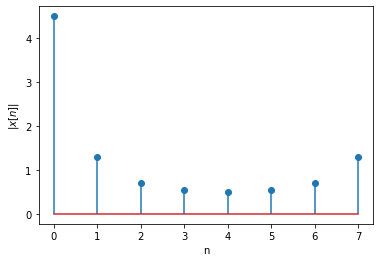
\includegraphics[width=\columnwidth] {fig.png}
    \caption{Magnitude of $x\sbrak{n}$ vs $n$}
\end{figure}
\end{document}
